\documentclass[a4paper, 12pt]{article}

% Package digunakan dalam dokumen laporan dan constraint
\usepackage[a4paper, margin=1in]{geometry}
\usepackage{tabularx}
\usepackage[utf8]{inputenc}
\usepackage{graphicx}
\usepackage{booktabs}
\usepackage{array}
\usepackage[bahasa]{babel}
\usepackage{setspace}
\onehalfspacing
\usepackage{float}
\usepackage{enumitem}

%awal 
\begin{document}

%Halman Judul 
\begin{titlepage}
    \centering
    \vspace*{\stretch{1.0}}
    
    {\Huge\bfseries Laporan Ujian Tengah Semester\par}
    \vspace{0.5cm}
    {\LARGE\bfseries Keamanan, Kesehatan, Keselamatan, dan Lingkungan Kerja Industri (K3L)\par}
    
    \vspace{2.5cm}
    %logo itera 
    \begin{figure}[htbp] 
        \centering
        \includegraphics[width=0.4\linewidth]{Logo_ITERA.png}
        \label{fig:logo}
    \end{figure}
    {\large Disusun oleh:\par}
    \vspace{0.5cm}
    {\Large Nama Mahasiswa: Daniel Calvin Simanjuntak\par}
    {\Large NIM: 123140004\par}
    
    \vspace{\stretch{2.0}}    
    {\large\bfseries Program Studi Teknik Informatika\par}
    {\large\bfseries Institut Teknologi Sumatera\par}
    \vspace{0.5cm}
    {\large Dosen Penguji:\par}
    {\large Amrina Mustaqim, S.Si., M.T.\par}
    {\large Hesti Wahyu Handani, S.Si., M.Si.\par}
    \vspace{0.5cm}
    {\large \today\par} 
    \vspace*{\stretch{1.0}}
\end{titlepage}



%Bab 1 
\section{Konsep dan Peran K3L}
\noindent\textbf{Judul Kasus:} Analisis Risiko dan Mitigasi Bahaya Fisik di Lingkungan Kampus Pada Jalan Penyeberangan antara Gedung E dan GK 2 ITERA 

\subsection{Deskripsi Situasi}
Pada area yang diamati yaitu Jalan Penyeberangan Gedung E ke Gedung Kuliah 2 (GK2), diidentifikasi adanya potensi bahaya fisik akibat tidak tersedianya
fasilitas keselamatan yang memadai. Fasilitas yang kurang yaitu marka jalan seperti \textit{zebra-cross} dan rambu lalu lintas tanda penyeberangan jalan.
Kondisi ini memungkinkan terjadinya insiden, dimana pejalan kaki berisiko tersenggol atau tertabrak kendaraan yang melintas.
\subsection{Analisis Konsep K3L}
Konsep K3L digunakan agar terciptanya lingkungan kerja yang aman, sehat, dan bebas dari kecelakaan. 
Dalam hal ini, konsep K3L diaplikasikan sebagai berikut:
\begin{itemize}
    \item \textbf{Keselamatan (Safety):} Fokus utama adalah melindungi seluruh warga kampus dari potensi kecelakaan. Tidak adanya \textit{zebra cross} merupakan 
      salah satu kekurangan pada aspek keselamatan yang dapat menyebabkan cedera fisik.
    \item \textbf{Kesehatan (Health):} Potensi kecelakaan dapat menimbulkan dampak kesehatan jangka panjang, baik fisik (cacat) maupun psikologis (trauma).
    \item \textbf{Proaktif dan Preventif:} Penerapan K3L yang efektif tidak harus ketika bahaya terjadi (reaktif), melainkan mengidentifikasi potensi bahaya (proaktif) dan 
      melakukan tindakan pencegahan (preventif) untuk menghilangkan atau mengurangi risiko.
\end{itemize}

\subsection{Peran K3L di Industri}
Peran K3L di sini adalah sebagai berikut:
\begin{enumerate}
    \item \textbf{Identifikasi dan Pengendalian Risiko:} Mengidentifikasi potensi-potensi bahaya yang ada di lingkungan kampus secara sistematis, serta merancang pengendalian bahayanya.
    \item \textbf{Pemenuhan Regulasi:} Setiap fasilitas dan kegiatan di lingkungan kampus harus memenuhi kriteria minimum kesalamatan dan peraturan yang ada.
    \item \textbf{Pembangunan Budaya Keselamatan:} Menciptakan budaya dan perilaku yang memperhatikan keselamatan pada lingkungan kampus. 
\end{enumerate}

\subsection{Strategi Komunikasi}
Strategi komunikasi yang jelas dan terstruktur diperlukan untuk melaksanakan prosedur ini, dari pelaporan dengan data, sosialisasi risiko, dan pelaporan kepada manajamen K3L.
%Bab 2 
\section{Regulasi dan Standar K3L}
\noindent\textbf{Judul Kasus:}  Analisis Risiko dan Mitigasi Bahaya Fisik di Lingkungan Kampus Pada Jalan Penyeberangan antara Gedung E dan GK 2 ITERA 

\subsection{Analisis Keterkaitan Regulasi}
Kondisi bahaya pada kasus ini relevan dengan beberapa regulasi dan standar K3L, antara lain:
\begin{itemize}
    \item \textbf{Undang-Undang No. 1 Tahun 1970 tentang Keselamatan Kerja:} Pasal 3 Ayat (1) mewajibkan pencegahan dan pengurangan kecelakaan. Pihak pengelola (universitas) berkewajiban menyediakan lingkungan yang aman.
    \item \textbf{ISO 45001:2018 (Sistem Manajemen K3):} Sesuai Klausul 6.1.2, organisasi wajib mengidentifikasi bahaya, menilai, dan mengendalikan risiko K3L secara proaktif.
\end{itemize}

\subsection{Langkah Perbaikan Sistem}
Perbaikan secara sistematis dapat dilakukan menggunakan \textit{Plan-Do-Check-Act} (PDCA):
\begin{description}
    \item[Plan] Merancang solusi teknis (spesifikasi \textit{zebra cross}, rambu) serta merencanakan anggaran dan jadwal implementasi.
    \item[Do] Melakukan instalisasi dari solusi teknis sesuai dengan desain yang telah disetujui.
    \item[Check] Melakukan pemantauan dan evaluasi efektivitas fasilitas setelah proses instalasi.
    \item[Act] Melakukan tindakan berupa solusi tambahan jika diperlukan (sesuai dengan keadaan), seperti penambahan \textit{speed bump}.
\end{description}

\subsection{Peran Komunikasi \& Pelatihan}
Komunikasi penting agar informasi rencana penanggulangan risiko dapat diketahui oleh civitas kampus. 
Pelatihan atau sosialisasi berguna untuk melatih dan mengedukasi civitas kampus tentang pentingnya keselamatan dalam melaksanakan suatu kegiatan atau menggunakan fasilitas kampus.

%Bab 3 
\section{Identifikasi Bahaya dan Analisis Risiko}

\subsection{Identifikasi Jenis Bahaya}
Jenis bahaya dari bahaya ini adalah adalah \textbf{Bahaya Fisik}. Bahaya ini berasal dari kendaraan yang melintas dan
fasilitas keselamatan yang kurang memadai.
\subsection{Analisis Risiko}

\begin{table}[H]
    \centering
    \caption{Tabel Analisis Risiko pada Area Penyeberangan Gedung E ke GK2}
    \label{tab:risiko}
    \fontsize{8pt}{10pt}\selectfont
    \begin{tabularx}{\textwidth}{>{\centering\arraybackslash}p{0.7cm} 
                                   >{\centering\arraybackslash}p{1.3cm} 
                                   >{\raggedright\arraybackslash}p{2.5cm} 
                                   >{\raggedright\arraybackslash}p{2.2cm} 
                                   >{\centering\arraybackslash}p{1.1cm} 
                                   >{\centering\arraybackslash}p{1.1cm} 
                                   >{\centering\arraybackslash}p{1.2cm} 
                                   >{\raggedright\arraybackslash}X}
        \toprule
        \textbf{No} & \textbf{Jenis Bahaya} & \textbf{Sumber Bahaya} & \textbf{Potensi Akibat} & \textbf{Nilai\ Kemung\-kinan} & \textbf{Nilai\ Kepa\-rahan} & \textbf{Tingkat Risiko} & \textbf{Rekomendasi Pengendalian} \\
        \midrule
        1 & Fisik & Kontak fisik dari pejalan kaki dan kendaraan di penyeberangan tanpa fasilitas keselamatan & 
        Cedera ringan, cedera berat, dan menyebabkan kematian.
        & 4 & 4 & 16 (Tinggi) & 
        \textbf{1.} Rekayasa Teknik: Pemasangan zebra cross, rambu lalu lintas, dan speed bump. 
        \newline
        \textbf{2.} Administratif: Sosialisasi pentingnya keselamatan dan penetapan batas kecepatan di lingkungan kampus. \\
        \bottomrule
    \end{tabularx}
\end{table}

\subsection{Alat Bantu Identifikasi Bahaya}
Metode atau alat bantu yang digunakan untuk mengidentifikasi bahaya ini adalah :
\begin{enumerate}
    \item \textbf{Inspeksi Keselamatan (\textit{Safety Inspection}):} Melakukan pengamatan dan pengumpulan data secara langsung di lokasi potensi bahaya.
    \item \textbf{Laporan Bahaya (\textit{Hazard Reporting}):} Menggunakan sistem pelaporan agar civitas kampus dapat melaporkan potensi bahaya yang ditemukan.
\end{enumerate}


%Bab 4 
\section{Penerapan SOP \& Sikap Akademik}

\subsection{Rancangan Singkat SOP untuk kasus yang telah anda pilih}

\begin{table}[H]
    \centering
    \caption{SOP: Prosedur Aman Menyeberang Jalan di Area Kampus}
    \label{tab:sop}
    \begin{tabularx}{\textwidth}{>{\centering\arraybackslash}p{1.5cm} 
                                  >{\raggedright\arraybackslash}X 
                                  >{\centering\arraybackslash}p{3cm} 
                                  >{\centering\arraybackslash}p{3cm}}
        \toprule
        \textbf{Langkah} & \textbf{Deskripsi Tindakan} & \textbf{Penanggung Jawab} & \textbf{Alat yang Digunakan} \\
        \midrule
        1 & Berhenti di tepi jalan,kemudian pastikan keadaan sekitar. & Pejalan Kaki & - \\
        \addlinespace
        2 & Lihat ke arah kanan dan kiri untuk memastikan tidak ada kendaraan yang mendekat.\ Jika terdapat kendaraan, gunakan tangan dengan
          mengangkat tangan untuk memberikan tanda ingin menyeberang kepada pengemudi kendaraan yang melintas. & Pejalan Kaki & Mata (Penglihatan) dan Tangan \\
        \addlinespace
        3 & Gunakan \textit{zebra cross} untuk menyeberang. & Pejalan Kaki & Fasilitas \textit{Zebra Cross} \\
        \addlinespace
        4 & Tetap waspada terhadap lalu lintas selama menyeberang. & Pejalan Kaki & - \\
        \bottomrule
    \end{tabularx}
\end{table}

\subsection{Sikap Akademik dan Komunikatif}
Dalam menjalankan lingkungan yang aman, penerapan sikap akademik dan komunikatif sangat penting. Sikap ini diwujudkan melalui:
\begin{itemize}
    \item \textbf{Sikap Analitis:} Menguraikan masalah secara sistematis dan detail (identifikasi bahaya, analisis risiko) dan tidak hanya menyampaikan keluhan umum.
    \item \textbf{Sikap Solutif:} Mengusulkan atau merancang solusi pasti dan berlapis berdasarkan hierarki pengendalian risiko.
    \item \textbf{Sikap Bertanggung Jawab:} Berinisiatif melaporkan temuan demi keselamatan civits kampus.
    \item \textbf{Sikap Komunikatif:} Menyajikan data dan analisis dalam format yang formal, jelas, dan persuasif kepada pihak berwenang.
\end{itemize}
\section{Lampiran}
\begin{enumerate}
  \item Gambar Kondisi 

  \begin{figure}[H]
    \centering
    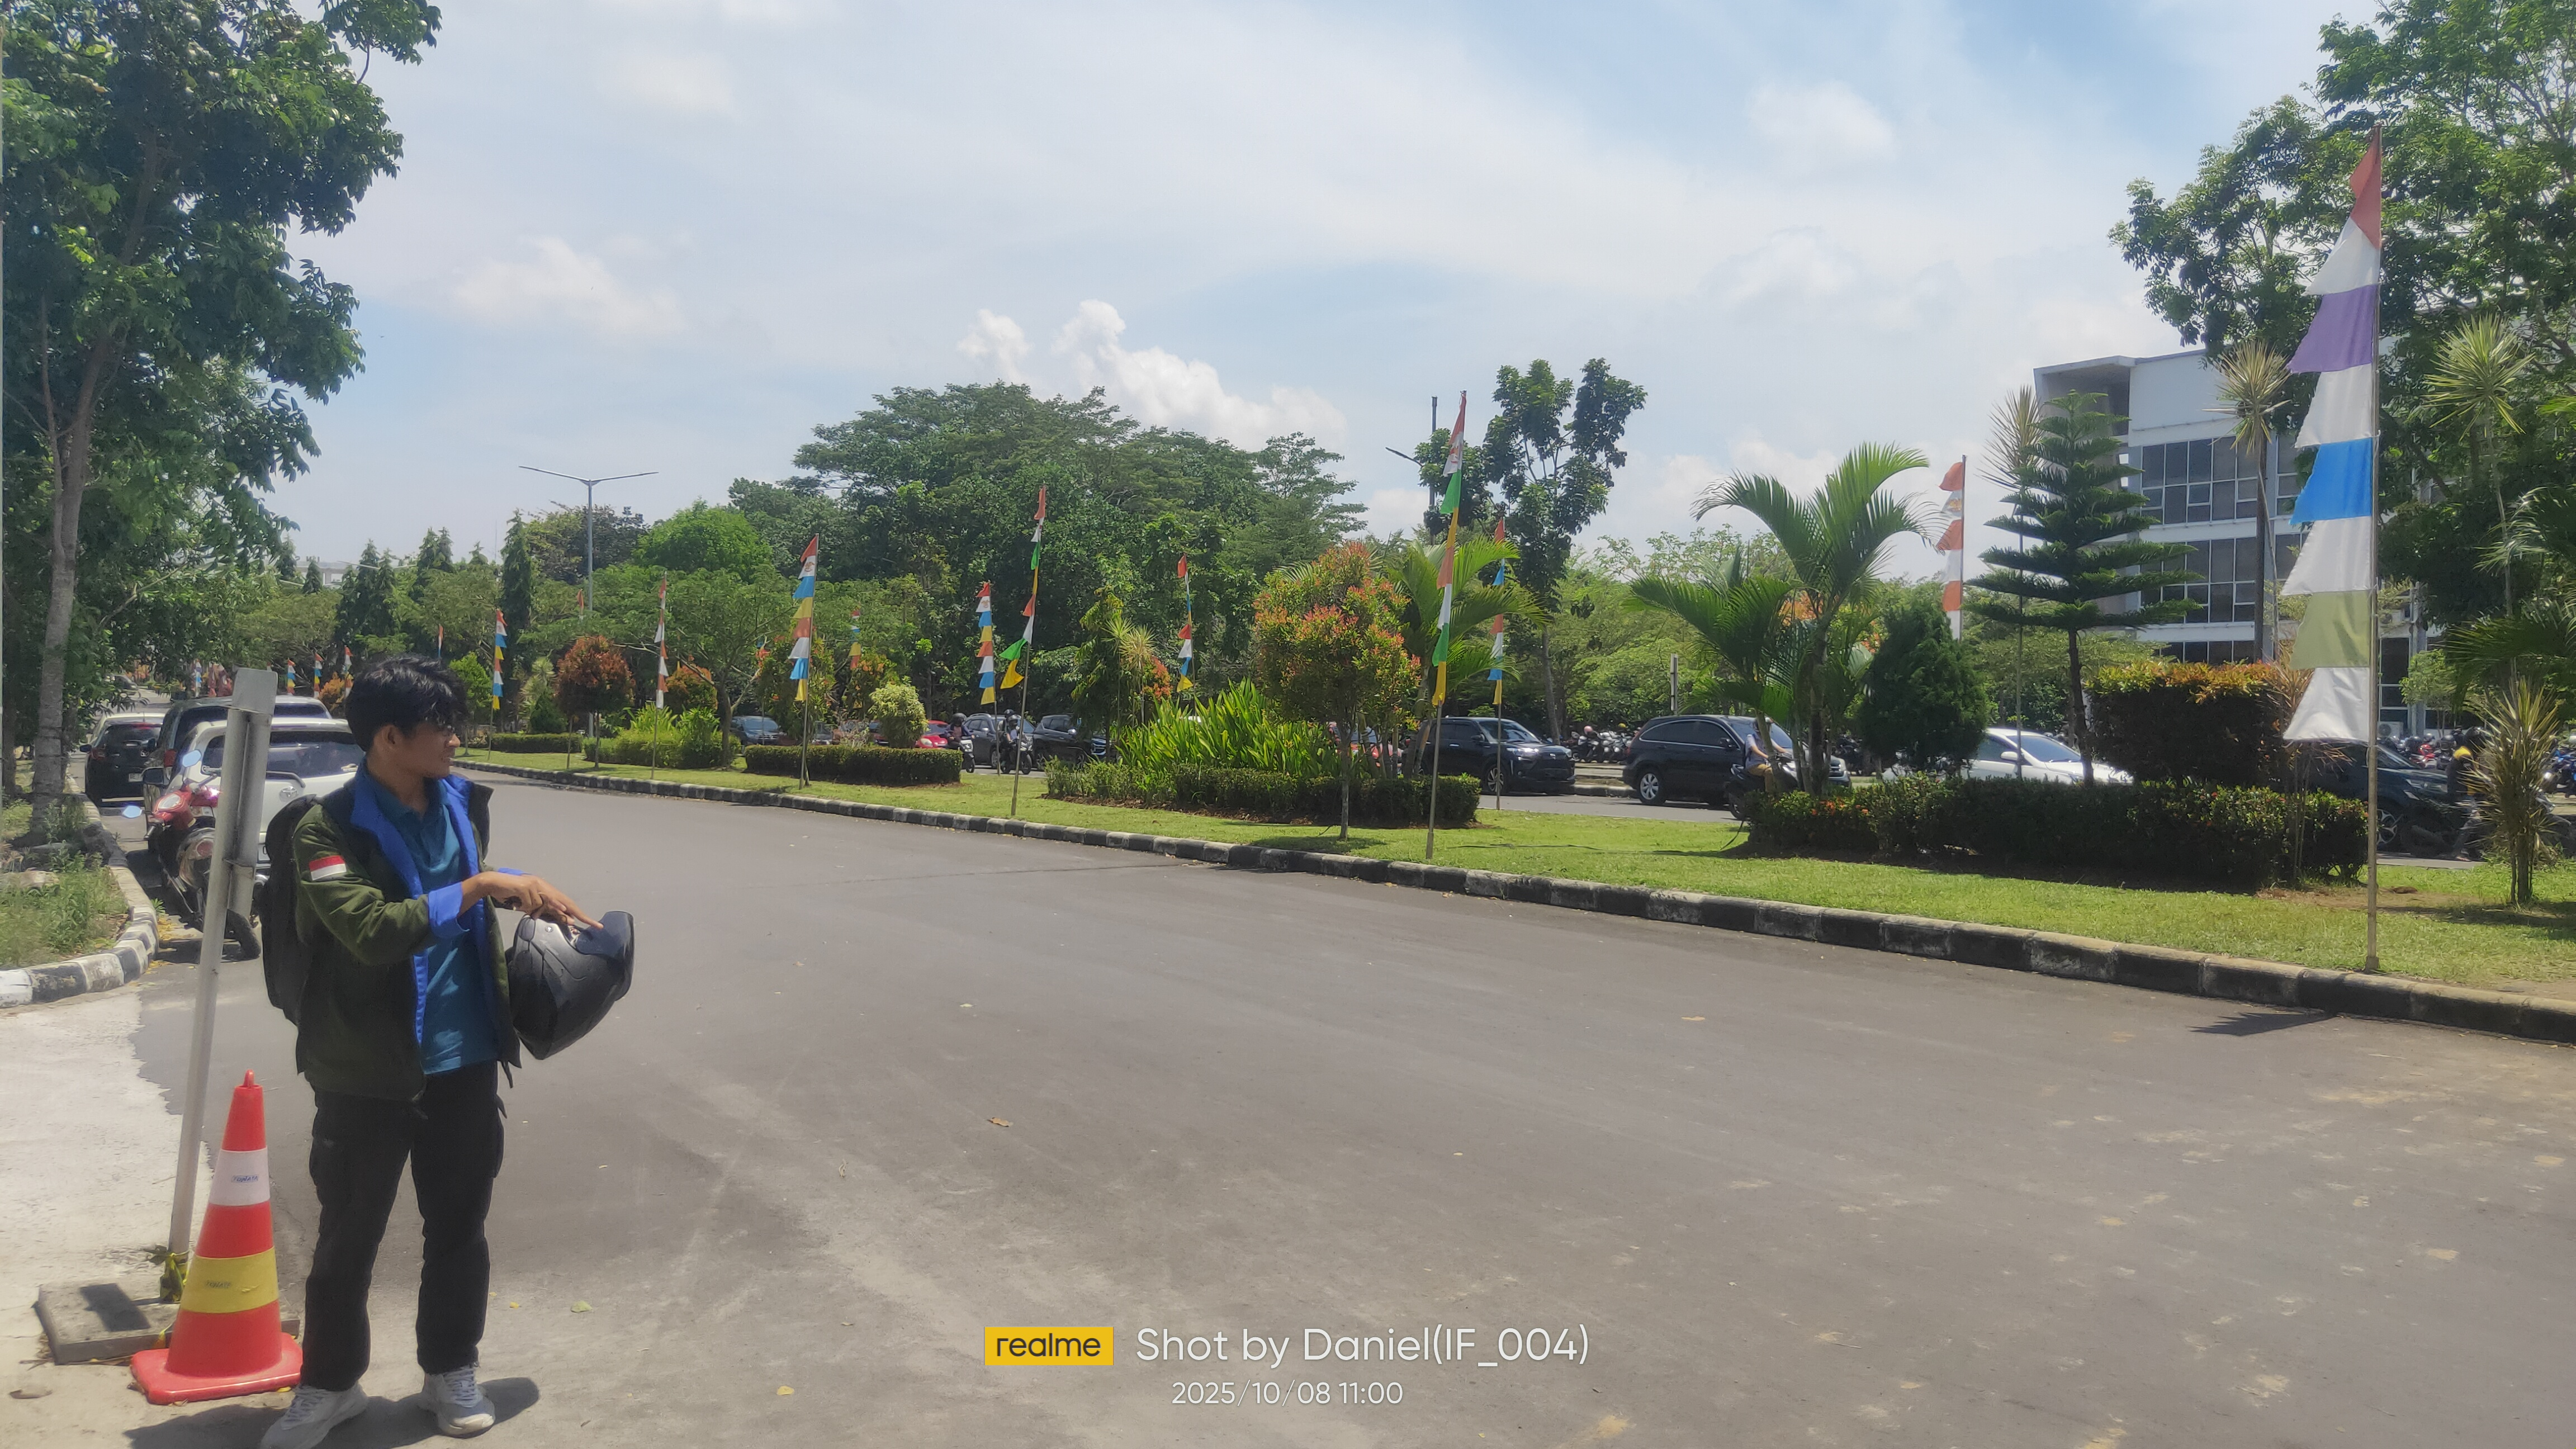
\includegraphics[width = .5\linewidth]{kondisi_lapangan_new.png}
    \caption{Kondisi Lapangan}
  \end{figure}  
\item Link repository GitHub : \url{https://github.com/daniel-got/Laporan-Analisis-Bahaya-with-LaTeX}

\end{enumerate}

% %-- AKHIR DOKUMEN --% %
\end{document}
